\chapter{StoryBoarding}

Dopo aver concluso il needfinding ed aver individuato i vari task su cui concentrarsi, 
il passo successivo è la realizzazione dei vari storyboard. 
Qui sotto verranno illustrati tre StoryBoarding con i relativi task.

\section{StoryBoarding 1: Condivisione di Appunti}

\subsection{Task}
\begin{enumerate}
    \item Ricercare il nome del corso desiderato
    \item Selezioni il corso d’interesse
    \item Ricerca l’argomento di quel corso su cui ti servono appunti
    \item Visualizza gli appunti su quell’argomento postati da altri studenti (eventualmente ordinati in base alle recensioni di altri studenti)  
\end{enumerate}

\subsection{StoryBoard}
\begin{center}
    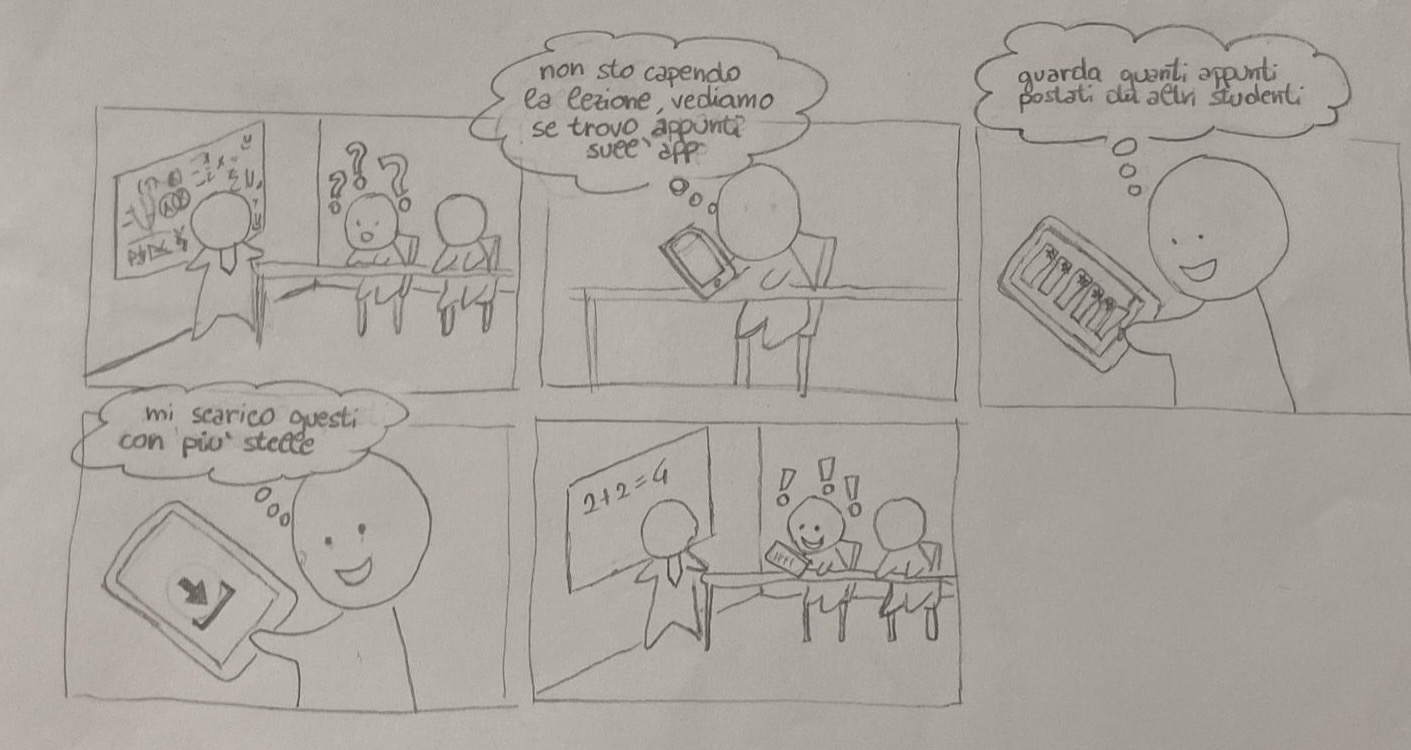
\includegraphics[width=1.1\textwidth]{/Users/leonardvincentramil/Desktop/MyDoc/MyLatex/ProgettoINTRUSIACSAI/02_StoryBoarding/img/SB1.jpg}
\end{center}

\section{StoryBoarding 2: Conoscere meglio il Professore}

\subsection{Task}
\begin{enumerate}
    \item Ricercare il nome del professore di tuo interesse
    \item Seleziona il professore desiderato
    \item Visualizza le informazioni di tuo interesse tra quelle disponibili riguardanti il professore
    \item Naviga sulle recensioni e/o sui commenti postati da altri studenti 
    \item Visualizza il suo curriculum vitae 
\end{enumerate}

\subsection{StoryBoard}
\begin{center}
    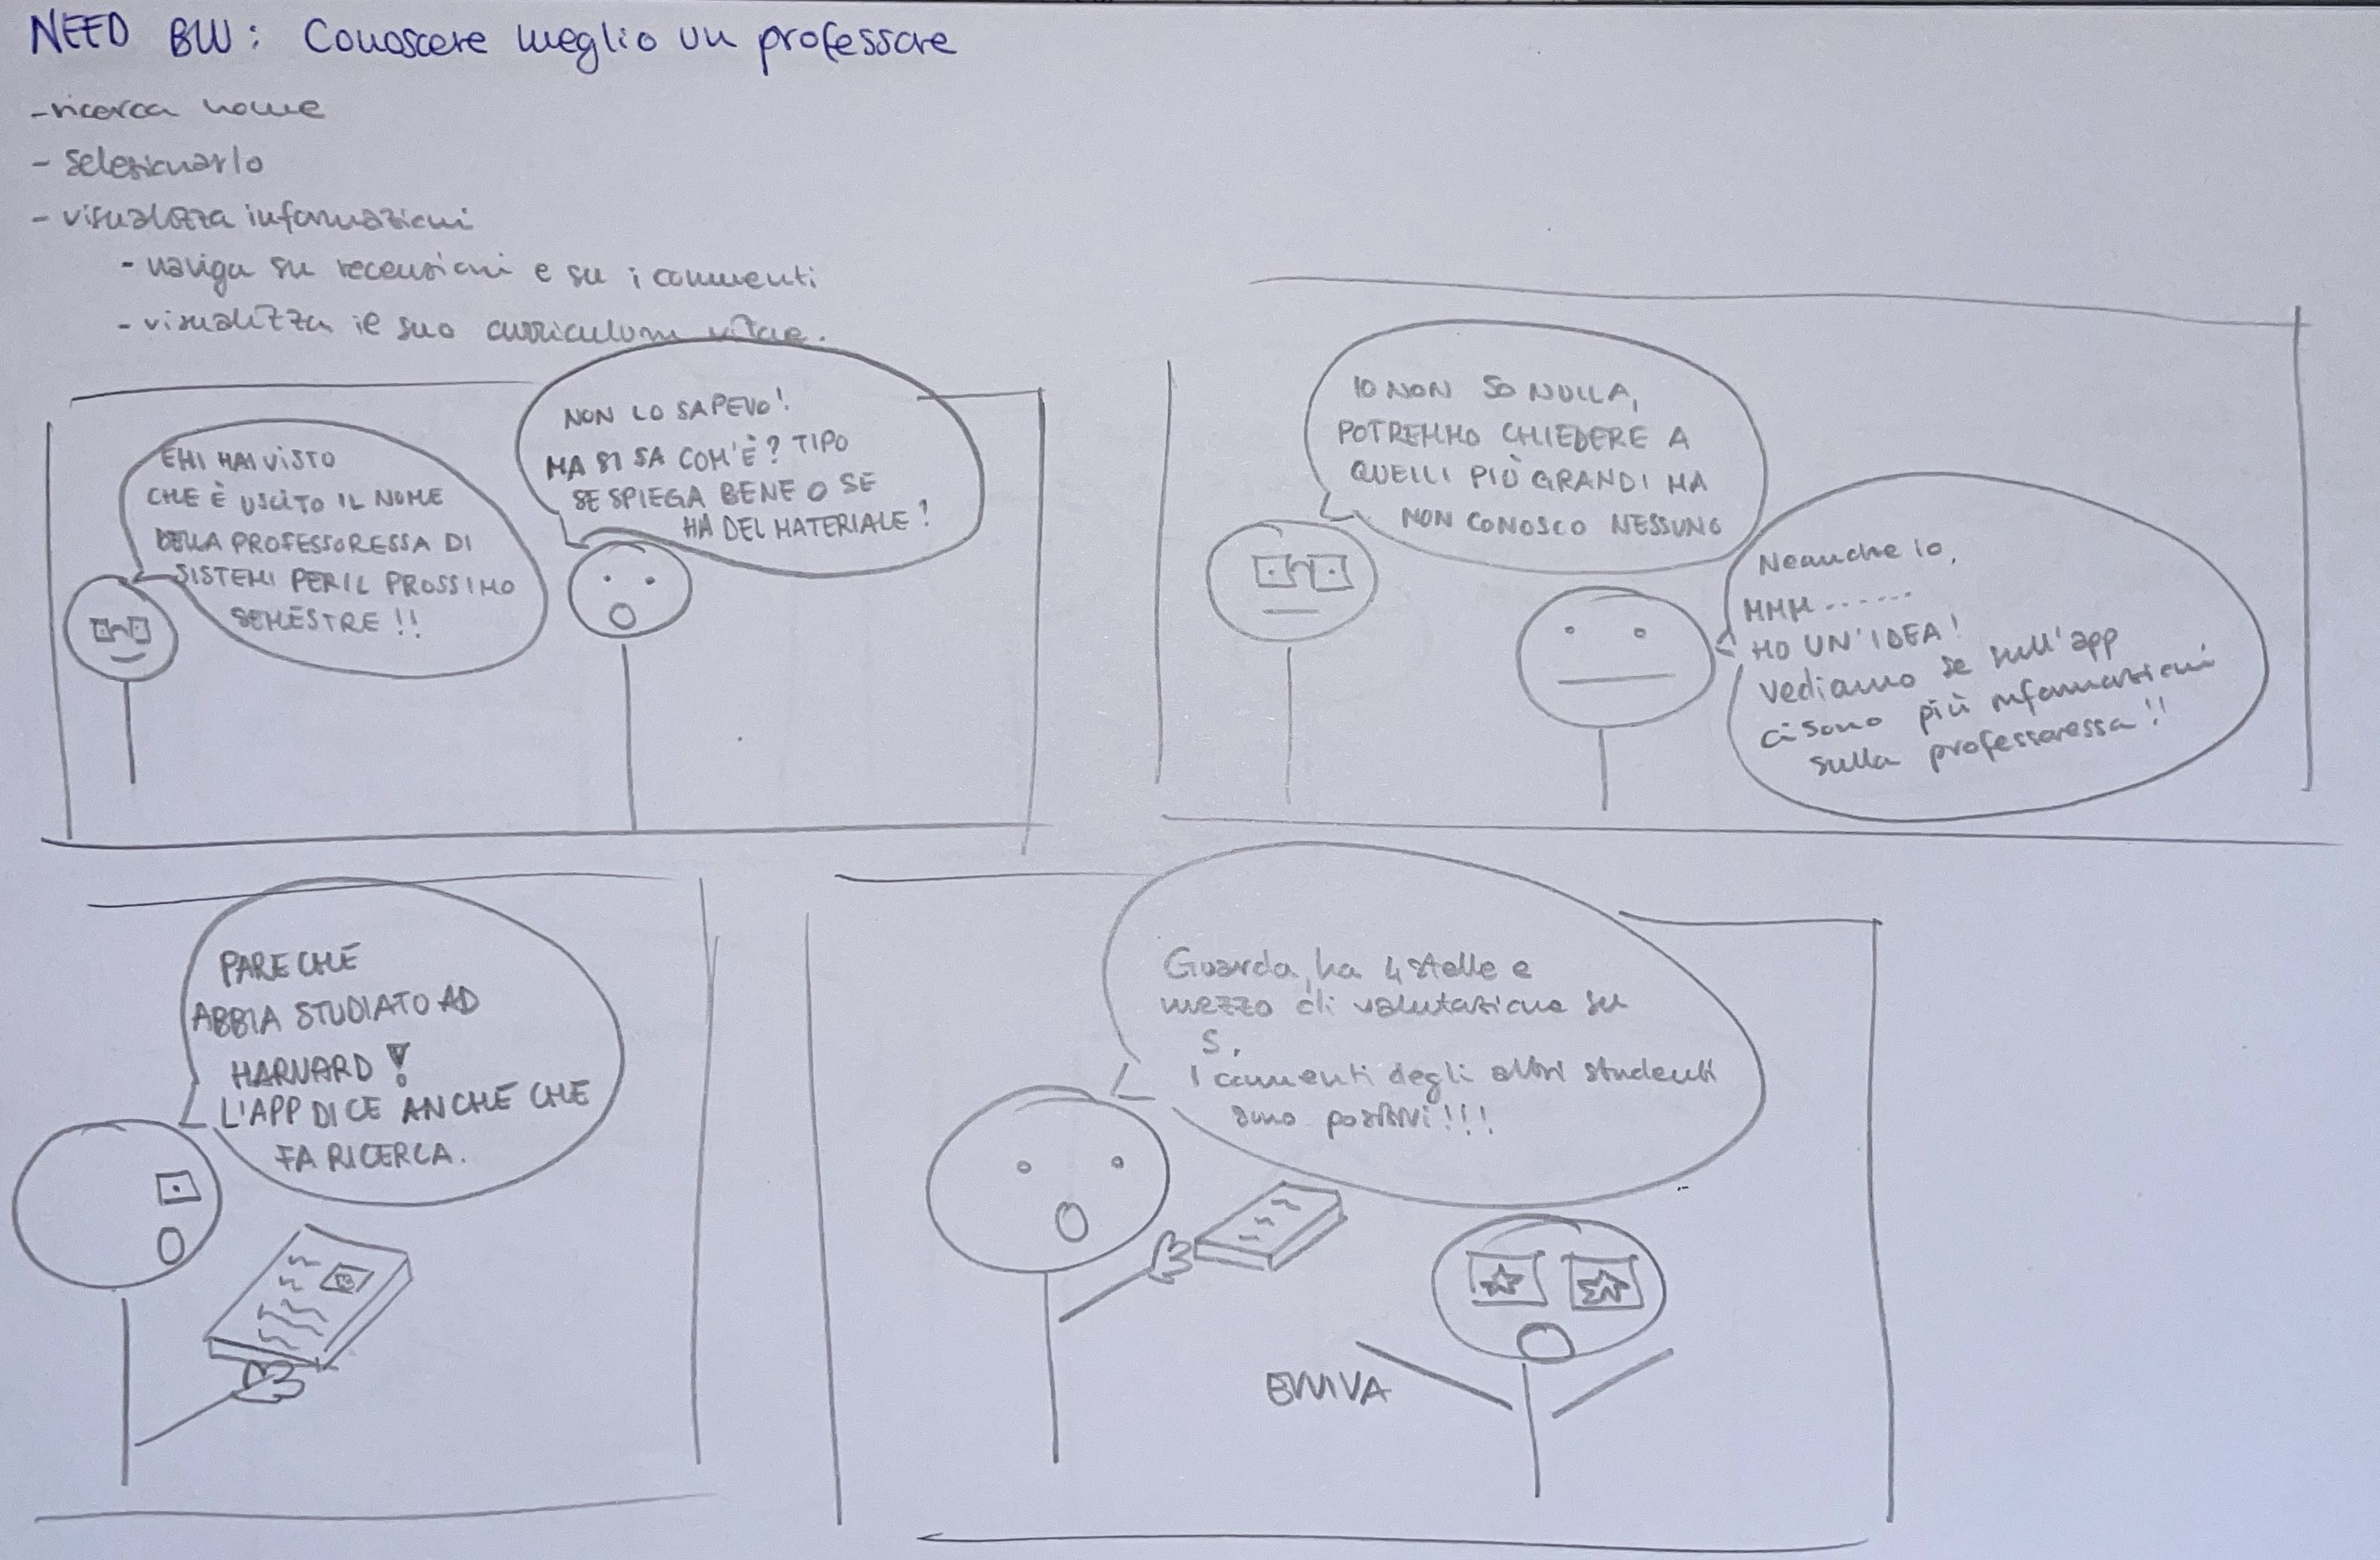
\includegraphics[width=1.1\textwidth]{/Users/leonardvincentramil/Desktop/MyDoc/MyLatex/ProgettoINTRUSIACSAI/02_StoryBoarding/img/SB2.jpg}
\end{center}


\section{StoryBoarding 3: Informarsi sul Tirocinio}

\subsection{Task}
\begin{enumerate}
    \item Ricercare il nome del professore di tuo interesse
    \item Seleziona il professore desiderato
    \item Visualizza le informazioni di tuo interesse tra quelle disponibili riguardanti il professore
    \item Naviga sui tirocini disponibili del professore cercato
\end{enumerate} 

\subsection{StoryBoard}
\begin{center}
    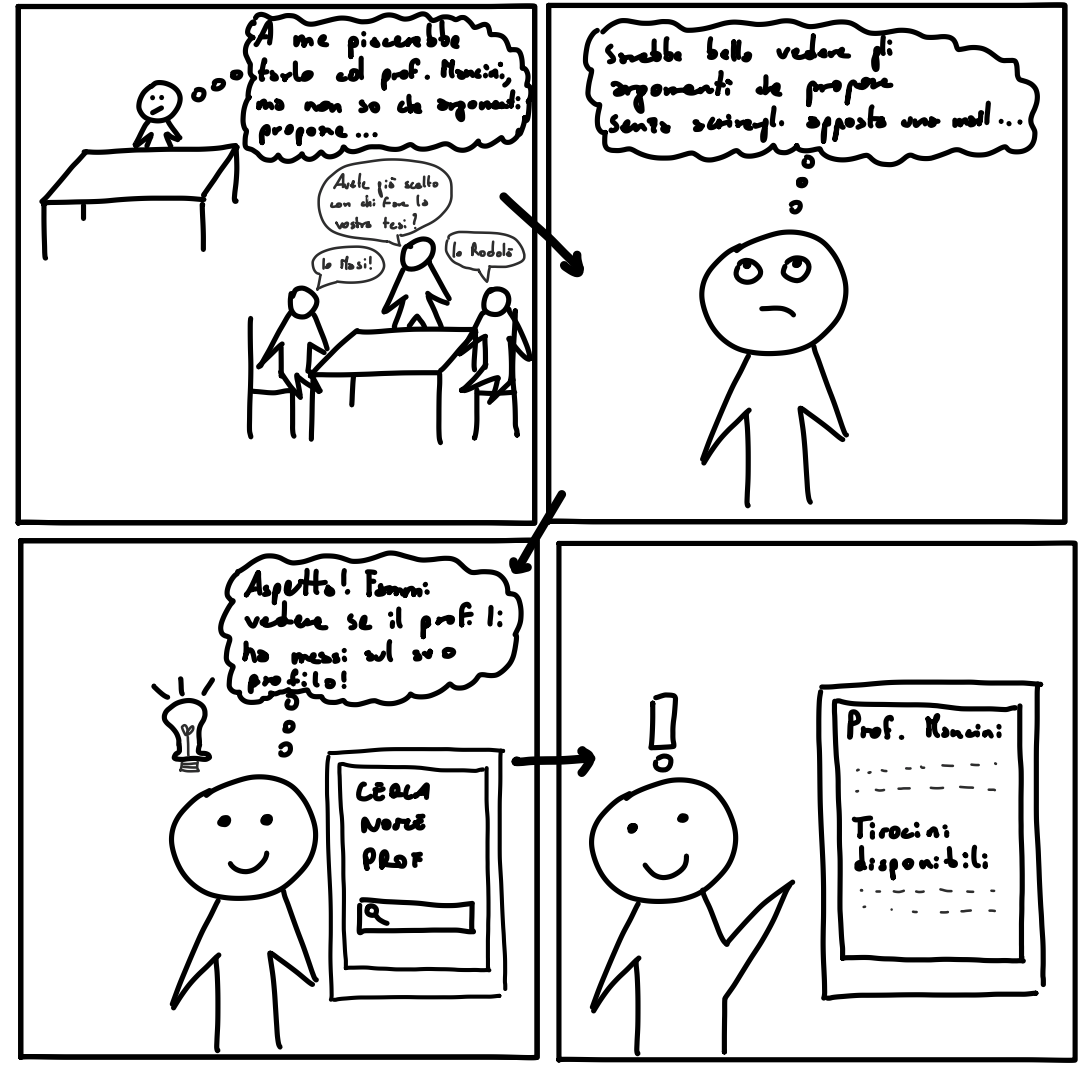
\includegraphics[width=1.1\textwidth]{/Users/leonardvincentramil/Desktop/MyDoc/MyLatex/ProgettoINTRUSIACSAI/02_StoryBoarding/img/SB3.png}
\end{center}
